Knihovna \texttt{tnums} v této chvíli umí přidávat racionální čísla, Ludolfovo číslo a provádět mezi nimi multiplikativní a aditivní operace. Bylo by vhodné teď přidat další rekurzivní čísla. Jejich dobrým zdrojem, jak jsem napsal již v~podkapitole \ref{funkce_cisel}, jsou matematické funkce. V této kapitole se podíváme na funkci exponenciální, šest funkcí goniometrických a přirozený logaritmus. Na konci potom dodělám matematické operace a tím bude knihovna v použitelné verzi hotová.

\subsection{Aproximace funkcí}
Představa funkce tnumu je, že bude opět vracet tnum. Chci totiž opět libovolnou přesnost a také umožnit zřetězování funkcí. Hledám pak formu aproximace, která bude umožňovat libovolně škálovat, jak blízko ke kýženému číslu se výpočet ukončí. Dobrým nástrojem k tomu jsou Taylorovy polynomy. Ty se snaží hledat hodnotu $T(x)$ tak, aby byla co nejblíže hledané hodnotě $f(x)$ tak, že z~nějakého bodu, kterému budeme říkat počátek, se co nejlépe snaží nepodobit průběh funkce, kterou aproximují. Pro funkci $f$ budu Taylorův polynom stupně $n$ se středem v $a$ značit $T^{f,a}_n$. Pro práci s Taylorovými polynomy potřebujeme ještě naprogramovat faktoriál přirozeného čísla. To bývá typická úloha na rekurzi -- té se ale vyhýbáme, protože pro velké vstupy může přetékat zásobník. Iterativní verze by tímto neduhem neměla trpět.

\begin{lispcode}{\texttt{factorial}}{Funkce pro výpočet faktoriálu přirozeného čísla}
(\textcolor{funkcionalni}{defun} \textcolor{pojmenovan}{factorial} (n)
  (\textcolor{vedlejsi}{let} ((result 1))
    (\textcolor{funkcionalni}{loop} \textcolor{obarvi}{for} i \textcolor{obarvi}{from} n \textcolor{obarvi}{downto} 1
          \textcolor{obarvi}{do} (\textcolor{vedlejsi}{setf} result (\textcolor{matematicke}{*} result i)))
    result))
\end{lispcode}

Podívejme se teď na to, jak se prakticky dá počítat aproximace funkce v bodě $x$. Nejjednodušší je vzít funkci $T^{f,a}_0(x) = f(a)$. Je to jednoduchá aproximace, která na velmi blízkém okolí bodu $a$ může fungovat i velmi uspokojivě. Lepší nápadem je vzít přímku, která se bude dotýkat grafu funkce $f$ v bodě $a$. Předpis takovéto bude $T^{f,a}_1(x) = f(a)+f'(a)(x-a)$. To už je lepší aproximace, protože nebere v úvahu jen hodnotu funkce $f$ v bodě $a$ ale i její první derivaci, takže víme více o směru, kam se možná bude pohybovat. Ještě lepším nápadem pak je vzít parabolu přimknutou k grafu funkce $f$ jako $T^{f,a}_2(x) = f(a)+f'(a)(x-a)+\frac{f''(a)}{2}(x-a)^2$. Teď už zohledňujeme funkční hodnotu, směr křivky i konvexnost. Ještě lepším nápadem je použít $T^{f,a}_3(x):y=f(a)+f'(a)(x-a)+\frac{f''(a)}{2}(x-a)^2+\frac{f'''(a)}{6}(x-a)^3\ldots$\cite{MTTP}.

\begin{remind}[Taylorova a Maclaurinova řada]
Kdybychom takto postupovali donekonečna (v limitním smyslu), dostali bychom Taylorovu řadu z definice \ref{def:taymac_rada}. Pro $a=0$ pak Taylorovu řadu nazýváme řadou Maclaurinovou.
\end{remind}

Lze odvodit, že pokud Taylorovy zbytky konvergují k nule, lze Taylorovou řadou $T_\infty^{f,a}$ nahradit funkci $f$ \cite{ZDVNNR}. Nám ale nestačí pouhá konvergence zbytků, ale chtěli bychom jejich velikost nějak omezovat. Nejprve si zkusme nějakou formou zbytky vyjádřit.

\begin{fact}[Taylorova věta \cite{TMA:Calculus}]
Nechť $f$ má spojité derivace až do řádu $n+1$ na nějakém intervalu obsahujícím $a$. Pak pro každé $x$ z tohoto intervalu máme Taylorův vzorec
\begin{equation}
f(x) = T_n^{f,a}(x) + R_n^{f,a}(x)\text{, kde}
\end{equation}
\begin{equation}\label{TP}
T_n^{f,a}(x) = \sum_{i=0}^{n}\frac{f{(i)}(a)}{i!}(x-a)^i,
\end{equation}
\begin{equation}\label{integralnitvar}
R_n^{f,a}(x)=\int_a^x\frac{(x-t)^n}{n!}f^{(n+1)}(t)dt.
\end{equation}
Navíc existuje číslo $\xi$, z intervalu s krajními body $x$ a $a$ takové, že
\begin{equation}\label{lagrangeuvtvar}
R_n^{f,a}(x)=\frac{f^{(n+1)}(\xi)}{(n+1)!}(x-a)^{n+1}.
\end{equation}
Pro důkaz vizte kapitolu 7.5 v \cite{TMA:Calculus}.
\end{fact}

Součet v rovnici \ref{TP} nazýváme Taylorův polynom funkce $f$ stupně $n$ v bodě $a$, $R_n^{f,a}(x)$ nazýváme $n$-tým Taylorovým zbytkem. Vyjádření \ref{integralnitvar} pak říkáme \textit{integrální tvar} zbytku a \ref{lagrangeuvtvar} je Lagrangeův tvar zbytku \cite{MTTP}.

Když už máme vyjádřeny zbytky, můžeme se pokusit je zhora omezovat, stejně jako tomu bylo u geometrické řady. Ve skutečnosti nám na celou kapitolu vystačí pouze tyto dva mechanismy, tedy \textit{Taylorův zbytek} a \textit{Zbytek geometrické řady}.

\subsection{Exponenciála}
Exponenciála je funkce s předpisem $\mathrm{exp}(x) = e^x$ kde $e$ je tzv. \textit{Eulerovo číslo} definované $e=\lim_{n\to\infty}\left(1+\frac{1}{n}\right)^n$ \cite{EPJVMAI}. To je transcendentní konstanta a je to též základ přirozeného logaritmu. Exponenciále se proto také dá říkat přirozená mocnina. Ještě podotkněme, že $\frac{d}{dx}\mathrm{exp}(x)=\mathrm{exp}(x)$.

\begin{myremark}{Značení exponenciály}
Mimo informatickou oblast jsem si nikde nevšiml, že by se exponenciála čísla $x$ značila jinak než $e^x$, mé značení $\mathrm{exp}(x)$ tedy možná působí neadekvátně. V dalším textu ale používám i pouze funkci ($\mathrm{exp}$), nikoli její hodnotu ($\mathrm{exp}(x)$) a předpis $e^x$ umožňuje jen toto druhé použití. Proto se omlouvám matematickému čtenáři za neintuitivní značení, ale je zde důvodné. Navíc lépe vyjadřuje, že je exponenciála funkcí.
\end{myremark}

\subsubsection{Exponenciála čísla}

\begin{fact}[Exponenciála jako Maclaurinova řada \cite{ZDVNNR}]\label{vet:exp_jako_rada}
Funkci $\mathrm{exp}(x)$ lze vyjádřit jako Maclaurinovu řadu ve tvaru
\begin{equation}
\mathrm{exp}(x) = \underset{i \in \mathbb{N}}{\sum} \frac{x^i}{i!} = \frac{1}{1} + \frac{x}{1} + \frac{x^2}{2!} + \frac{x^3}{3!} + \ldots
\end{equation}
\end{fact}

Podívejme se nyní na zbytek této řady. Když rozepíšeme Lagrangeův tvar, získáváme pro nějaké $\xi\in(0,x)$
\begin{equation}
R_n^{exp, 0}(x) = \frac{e^\xi}{(n+1)!}x^{n+1}.
\end{equation}

Podotkněme, že exponenciála je rostoucí a že $e<2.72$ a proto
\begin{equation}
(\forall\xi\in (0,x))(\mathrm{exp}(\xi)<\mathrm{exp}(x) < 2.72^x).
\end{equation}

Když vše poskládáme dohromady, získáváme aproximaci exponenciály na shora omezenou přesnost, pro $x\in\mathbb{R}$ platí
\begin{fact}[Omezení Taylorova zbytku exponenciály]
\begin{equation}
|R_n^{exp, 0}(x)| = \left|\mathrm{exp}(x)- \sum_{i=0}^n \frac{x^i}{i!}\right| \leq \left| \frac{2.72^x}{(n+1)!}x^{n+1} \right|.
\end{equation}
\end{fact}

\begin{consequence}[O tnumu exponenciály numu]
Pro všechna $\varepsilon$ existuje $n\in\mathbb{N}^+$ tak, aby $\left|\frac{2.72^x}{(n+1)!}x^{n+1}\right| \leq \varepsilon$ a nechť funkce $\tnum{}(x)$ má předpis
\begin{equation}
\tnum{}(x)(\varepsilon)=\sum_{i=0}^n \frac{x^i}{i!},
\end{equation}
pak $\tnum{}(x)\in\Tnum{\mathrm{exp}(x)},x\in\mathbb{Q}$.
\begin{proof}
Existence čísla $n$ je zřejmá z definice limity posloupnosti a z toho, že limita podílu polynomu a faktoriálu je rovna nule.

Dále protože $\mathrm{exp}(x) = T^{exp, 0}_n(x)+R^{exp, 0}_n(x)$, lze psát
\begin{equation}
T^{exp, 0}_n(x) \in [\mathrm{exp}(x) - |R^{exp, 0}_n(x)|, \mathrm{exp}(x) + |R^{exp, 0}_n(x)|],
\end{equation}
přičemž dle předchozího faktu platí
\begin{equation}
T^{exp, 0}_n(x) \in [\mathrm{exp}(x) - \left| \frac{2.72^x}{(n+1)!}x^{n+1} \right|, \mathrm{exp}(x) + \left| \frac{2.72^x}{(n+1)!}x^{n+1} \right|]
\end{equation}
a z předpokladu pak
\begin{equation}
T^{exp, 0}_n(x) \in [\mathrm{exp}(x) - \varepsilon, \mathrm{exp}(x) + \varepsilon].
\end{equation}
\end{proof}
\end{consequence}

Při implementaci stačí jen iterovat přes $n$, dokud nebude právě odvozené omezení zbytku menší než kýžená přesnost. Stejný přístup jsme viděli již u Ludolfova čísla.

\begin{lispcode}{\texttt{num-exp}}{Funkce pro výpočet exponenciály čísla na danou přesnost}
(\textcolor{funkcionalni}{defun} \textcolor{pojmenovan}{num-exp} (num eps)
  (\textcolor{vedlejsi}{let} ((above (\textcolor{moje}{rat-expt} 272/100 num)) (n 0)
        (nfact 1) (xpown 1) (result 1))
    (\textcolor{funkcionalni}{loop} 
     \textcolor{obarvi}{until} (\textcolor{matematicke}{<=} (\textcolor{matematicke}{/} (\textcolor{matematicke}{*} above xpown) nfact) eps)
     \textcolor{obarvi}{do} (progn
          (\textcolor{vedlejsi}{incf} n)
          (\textcolor{vedlejsi}{setf} nfact (\textcolor{moje}{factorial} n)
                xpown (\textcolor{matematicke}{expt} num n))
          (\textcolor{vedlejsi}{incf} result (\textcolor{matematicke}{/} xpown nfact)))
     \textcolor{obarvi}{finally} (\textcolor{funkcionalni}{return} result))))
\end{lispcode}

\begin{myremarkbez}{Eulerovo číslo jako exponenciála}
Protože triviálně platí $e = e^1$, můžu do knihovny přidat i samotné Eulerovo číslo jako jednoduchou uživatelskou funkci.
\begin{lispcode}{\texttt{tnum-e}}{Funkce pro tnum Eulerova čísla\hfill$\blacksquare$}
(\textcolor{funkcionalni}{defun} \textcolor{pojmenovan}{tnum-e} ()
  (\textcolor{funkcionalni}{lambda} (eps)
    (\textcolor{moje}{num-exp} 1 eps)))
\end{lispcode}
\end{myremarkbez}

Už tedy umíme exponenciálu čísla na danou přesnost. Teď jsme tedy ve stádiu, kdy lze pro $q\in\mathbb{Q}$ napsat
\begin{equation}
\texttt{(num-exp } q \texttt{)}\in\Tnum{\mathrm{exp}(q)}.
\end{equation}
To není malý výsledek, bohužel nás ale sotva uspokojí. Nyní ještě musíme rozšířit funkcionalitu na všechna reálná čísla, která mají tnum. Opět jde o linku rozdílu mezi racionálními a rekurzivními čísly, která prochází celou prací.

\subsubsection{Exponenciála tnumu}
Víme, že $\txe \in [x-\varepsilon,x+\varepsilon]$, podívejme se, jak se chová přesnost čísla po projití exponenciální funkcí.

\begin{myfigure}{H}
\caption{Obraz přesnosti po průchodu exponenciálou}
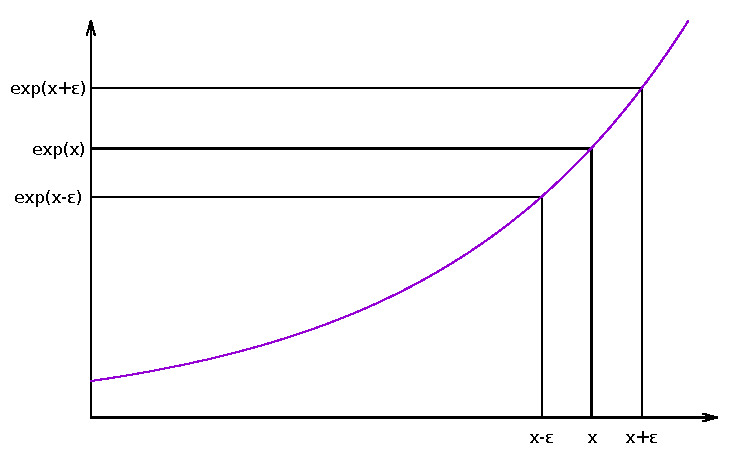
\includegraphics[width=\linewidth]{graphics/exp1.pdf}\label{fig:exp1}
Horní interval je vyšší než spodní.

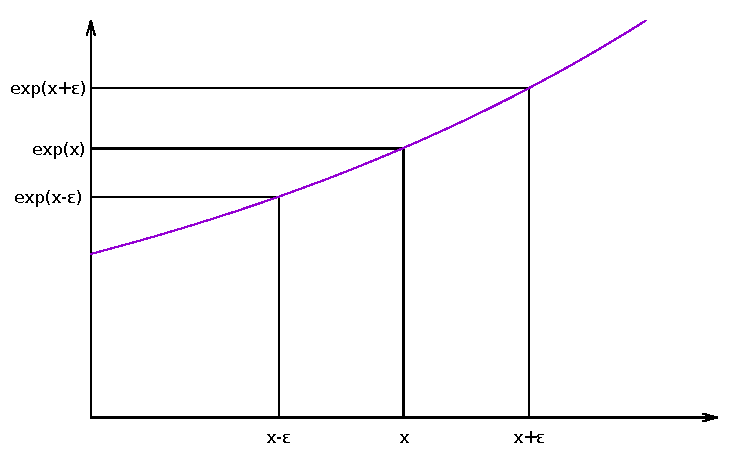
\includegraphics[width=\linewidth]{graphics/exp4.pdf}\label{fig:exp4}
Interval $[x-\varepsilon,x+\varepsilon]$ se nezobrazí na $[e^x-\varepsilon,e^x+\varepsilon]$. Tím pádem $\tnum{\mathrm{exp}(\txe)}\not\in\Tnum{\mathrm{exp}(x)},x\in\mathbb{R}$.
\end{myfigure}

Vidíme, že $|(x-\varepsilon)-x|=|(x+\varepsilon)-x|$, ale $|\mathrm{exp}(x-\varepsilon)-\mathrm{exp}(x)|\neq|\mathrm{exp}(x+\varepsilon)-\mathrm{exp}(x)|$, tedy že přesnost se průchodem nelineární funkcí deformuje a proto se interval $[\mathrm{exp}(x-\varepsilon),\mathrm{exp}(x+\varepsilon)]$ neshoduje s intervalem $[\mathrm{exp}(x)-\varepsilon,\mathrm{exp}(x)+\varepsilon]$. Důsledkem pak je, že nelze rozšířit funkce racionálních čísel na tnumy ve smyslu $\tnum{}(\varepsilon) := \tnum{\mathrm{exp}(\txe)}(\varepsilon)$, ale budeme to muset udělat šetrněji.

Pátráme po metodě, která nám řekne, jak přesné má být číslo na vstupu do funkce, aby jeho obraz byl v zadané přesnosti.

\begin{myfigure}{H}
\caption{Vzor přesnosti před průchodem exponenciálou}
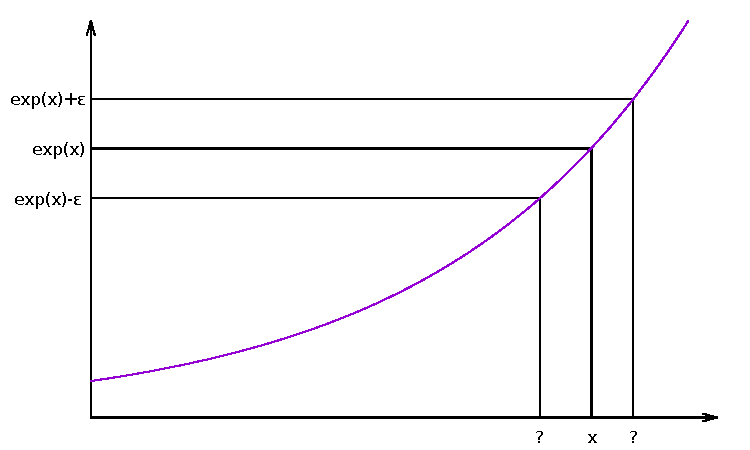
\includegraphics[width=\linewidth]{graphics/exp2.pdf}\label{fig:exp2}
Levý interval je širší než pravý.

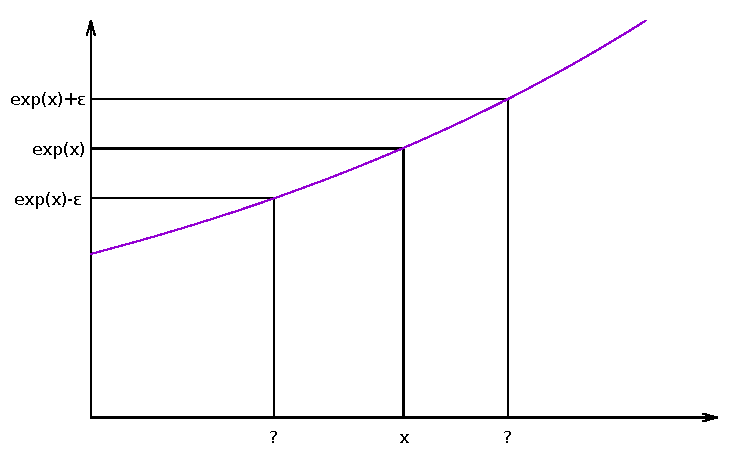
\includegraphics[width=\linewidth]{graphics/exp3.pdf}\label{fig:exp3}
Hledáme, jaké okolí bodu $x$ se zobrazí na $\varepsilon$-okolí bodu $e^x$.
\end{myfigure}

Když si to vyneseme do rovnice, bude vypadat
\begin{equation}\label{invpresexp}
\mathrm{exp}(x)+\varepsilon=\mathrm{exp}(x+w),
\end{equation}
kde hledaná neznámá je $w$.

\begin{myfigure}{H}
\caption{Zobrazení neznámé $w$}
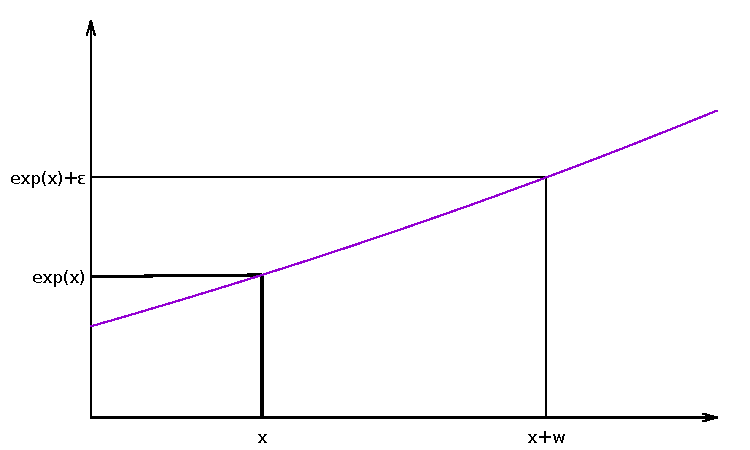
\includegraphics[width=.5\linewidth]{graphics/exp5.pdf}\label{fig:exp5}
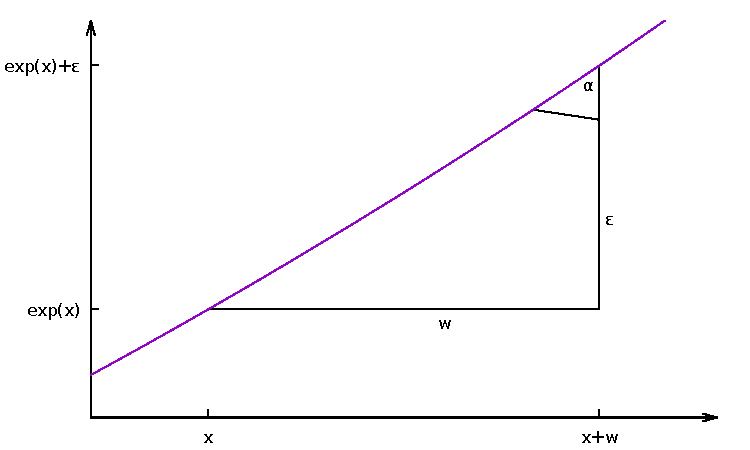
\includegraphics[width=.5\linewidth]{graphics/exp6.pdf}\label{fig:exp6}
Neznámou $w$ lze zobrazit jako jednu z odvěsen, druhá je $\varepsilon$. Fialová čára není přepona, ale exponenciála.
\end{myfigure}

Podívejme se nyní, jaký vztah je mezi $w$ a $\varepsilon$. Pro úhel $\alpha$ při vrcholu $W$ platí, že $\mathrm{ctan}(\alpha) = \frac{\varepsilon}{w}$. Tedy
\begin{equation}
w = \frac{\varepsilon}{\mathrm{ctan}(\alpha)} = \frac{\varepsilon}{\mathrm{tan}(\frac{\pi}{2}-\alpha)} = \frac{\varepsilon}{exp(x+w)}.
\end{equation}

Poslední úprava je přepsání skutečnosti, že tangens je v tomto bodě roven derivaci a derivace exponenciály je exponenciála. Vychází rekurzivní vztah pro $w$, po jeho dosazení do vztahu \ref{invpresexp} dostáváme
\begin{equation}\label{rekpresexp}
\mathrm{exp}(x)+\varepsilon=\mathrm{exp}\left(x+\frac{\varepsilon}{\mathrm{exp}\left(x+\frac{\varepsilon}{\mathrm{exp}(x+\ldots)}\right)}\right).
\end{equation}

Podobným způsobem lze odvodit i vztah pro opačný kraj okolí a to
\begin{equation}\label{rekpresexp2}
\mathrm{exp}(x)-\varepsilon=\mathrm{exp}\left(x-\frac{\varepsilon}{\mathrm{exp}\left(x-\frac{\varepsilon}{\mathrm{exp}(x-\ldots)}\right)}\right),
\end{equation}

dohromady to pak po propojení s notací tnumů dává vztah

\begin{equation}\label{rekpresexp3}
\tnum{\mathrm{exp}(x)}(\varepsilon)\in\left[
\mathrm{exp}\left(x-\frac{\varepsilon}{\mathrm{exp}\left(x-\frac{\varepsilon}{\mathrm{exp}(x-\ldots)}\right)}\right), \mathrm{exp}\left(x+\frac{\varepsilon}{\mathrm{exp}\left(x+\frac{\varepsilon}{\mathrm{exp}(x+\ldots)}\right)}\right)\right].
\end{equation}

\begin{myremarkbez}{Obecnější přesnost vzoru}
Odložím si zde obecnější trvzení, které vychází z právě dokázaného vztahu pro exponenciálu, jeho platnost by nyní měla být jasná pro všechny neklesající funkce spojité v $x$.
\begin{lemma}[O přesnosti závislé proměnné]\label{lem:presprom}
\begin{equation}\label{eq:presprom}
f(x)+\varepsilon=f(x+w)\text{,~kde~}w=f\left(x+\frac{\varepsilon}{f^{'}(x+w)}\right).
\end{equation}
\begin{proofscernou}
Tělo důkazu je již v řádcích a obrázcích nad tímto lemmatem. Protože $\varepsilon$ může být jakkoli malé, je úhel $\alpha$ roven derivaci v bodě $x+w$ a proto pak platí právě uvedený vztah.\hfill$\square\blacksquare$
\end{proofscernou}
\end{lemma}
\end{myremarkbez}

Z výše uvedených vztahů by mělo být jasné, že při implementaci budeme hledat pevný bod a proto si zavedeme tzv. \textit{precizní iterátor}.

\begin{definition}[Precizní iterátor exponenciály]
Definujme následující posloupnost:
\begin{equation}
\left[\tnum{x}\right]_0^{\mathrm{exp},\varepsilon}=\tnum{\mathrm{exp}(\txe)}(\varepsilon),
\end{equation}
\begin{equation}
\left[ \tnum{x}\right]_{n+1}^{\mathrm{exp},\varepsilon}=\tnum{\mathrm{exp}\left(\tnum{x}\left(\frac{\varepsilon}{\left|\left[ \tnum{x}\right]_n^{\mathrm{exp},\varepsilon}\right|+\varepsilon}\right)\right)}(\varepsilon)
\end{equation}
a pokud existuje $m$ tak, že
\begin{equation}
\left[\tnum{x}\right]_m^{\mathrm{exp},\varepsilon} = \left[\tnum{x}\right]_{m+1}^{\mathrm{exp},\varepsilon}\text{, pak klademe}\left[\tnum{x} \right]_\infty^{\mathrm{exp},\varepsilon} := \left[\tnum{x}\right]_m^{\mathrm{exp},\varepsilon}.
\end{equation}
\end{definition}

\begin{consequence}[O exponenciále tnumu]\label{dusl:expotnumu}
Nechť $\tnum{x}\in\Tnum{x},x\in\mathbb{R}$ a $\tnum{\mathrm{exp}(q)}\in\Tnum{\mathrm{exp}(q)},q\in\mathbb{Q}$ a funkce $\tnum{}(\tnum{x})$ má předpis
\begin{equation}
\tnum{}(\tnum{x})(\varepsilon)=\left[\tnum{x}\right]_\infty^{exp,\varepsilon},
\end{equation}
pak $\tnum{}(\tnum{x})\in\Tnum{\mathrm{exp}(x)},x\in\mathbb{R}$.
\begin{proof}
Vychází přímo ze vztahu \ref{rekpresexp3}.
\end{proof}
\end{consequence}

\begin{lispcode}{\texttt{tnum-exp}}{Funkce pro rozšíření funkcí z racionálních čísel na tnumy}
(\textcolor{funkcionalni}{defun} \textcolor{pojmenovan}{tnum-exp} (tnum)
  (\textcolor{funkcionalni}{lambda} (eps)
    (\textcolor{funkcionalni}{loop} \textcolor{obarvi}{for} i \textcolor{obarvi}{from} 0
          \textcolor{obarvi}{for} num = (\textcolor{funkcionalni}{if} (\textcolor{funkcionalni}{zerop} i) (\textcolor{moje}{tnum-to-num} tnum eps) new)
          \textcolor{obarvi}{for} new = (\textcolor{funkcionalni}{if} (\textcolor{funkcionalni}{zerop} i) 1
                      (\textcolor{funkcionalni}{if} (\textcolor{matematicke}{>} expnum 1)
                          (\textcolor{moje}{tnum-to-num} tnum (\textcolor{matematicke}{/} eps 
                                               (\textcolor{matematicke}{+} expnum eps)))
                        num))
          \textcolor{obarvi}{for} expnum = (\textcolor{moje}{num-exp} num eps)
          \textcolor{obarvi}{until} (\textcolor{matematicke}{=} num new) \textcolor{obarvi}{finally} (\textcolor{funkcionalni}{return} expnum))))
\end{lispcode}

\subsection{Goniometrické}
Goniometrické funkce jsou opět reálné funkce reálné proměnné. Poznamenejme, že $\frac{d}{dx}\mathrm{sin}(x) = \mathrm{cos}(x)$, $\frac{d}{dx}\mathrm{cos}(x) = -\mathrm{sin}(x)$ a že $H(\mathrm{sin}) = [-1,1] = H(\mathrm{cos})$.

\subsubsection{Sinus}
\begin{fact}[Sinus jako Maclaurinova řada \cite{ZDVNNR}]\label{vet:sin_jako_rada}
Funkci $\mathrm{sin}(x)$ lze vyjádřit jako Maclaurinovu řadu ve tvaru
\begin{equation}
\mathrm{sin}(x) =\sum_{i \in \mathbb{N}} (-1)^i \frac{x^{2i+1}}{(2i+1)!} =\frac{x}{1} - \frac{x^3}{3!} + \frac{x^5}{5!} - \frac{x^7}{7!} + \ldots
\end{equation}
\end{fact}

Dále protože jsou funkční hodnoty všech možných derivací v intervalu $[-1,1]$, lze Lagrangeův tvar zbytku vyjádřit bez znaménka a pak díky Taylorově větě platí
\begin{equation}
\left|\mathcal{R}^{sin, 0}_n(x)\right|\leq\left|\frac{x^{2n+1+1}}{(2n+1+1)!}\right|=\left|\frac{x^{2n+2}}{(2n+2)!}\right|.
\end{equation}

\begin{consequence}[Sinus numu]
Pro všechna $\varepsilon$ existuje $n\in\mathbb{N}^+$ tak, aby $\left|\frac{x^{2n+2}}{(2n+3)!}\right| \leq \varepsilon$ a nechť funkce $\tnum{}(x)$ má předpis
\begin{equation}
\tnum{}(x)(\varepsilon)=\sum_{i=0}^n (-1)^i \frac{x^{2i+1}}{(2i+1)!},
\end{equation}
pak $\tnum{}(x)\in\Tnum{\mathrm{sin}(x)},x\in\mathbb{Q}$.
\begin{proof}
Běží podobně jako u exponenciály. Jde opět o exponenciálu nad faktoriálem, proto je jasná limita i existence $n$. Dále z omezení $R^{\mathrm{sin}, 0}_n$ lze odvodit $T^{\mathrm{sin}, 0}_n\in[\mathrm{sin}(x)-|R^{\mathrm{sin}, 0}_n|,\mathrm{sin}(x)+|R^{\mathrm{sin}, 0}_n|]$ a pak $T^{\mathrm{sin}, 0}_n\in[\mathrm{sin}(x)-|\frac{x^{2n+2}}{(2n+2)!}|,\mathrm{sin}(x)+|\frac{x^{2n+2}}{(2n+2)!}|]$ a tudíž $T^{\mathrm{sin}, 0}_n\in[\mathrm{sin}(x)-\varepsilon,\mathrm{sin}(x)+\varepsilon]$, z čehož pak $\mathcal{T}^{\mathrm{sin}(x)}(\varepsilon)=T^{\mathrm{sin},0}_n(x)$.
\end{proof}
\end{consequence}

\begin{lispcode}{\texttt{num-sin}}{Funkce pro sinus čísla}
(\textcolor{funkcionalni}{defun} \textcolor{pojmenovan}{num-sin} (x eps)
  (\textcolor{vedlejsi}{let} ((result 0))
    (\textcolor{funkcionalni}{loop} \textcolor{obarvi}{for} n \textcolor{obarvi}{from} 0
          \textcolor{obarvi}{for} 2n+1 = (\textcolor{matematicke}{1+} (\textcolor{matematicke}{*} 2 n))
          \textcolor{obarvi}{do} (\textcolor{vedlejsi}{incf} result
                   (\textcolor{matematicke}{/} (\textcolor{moje}{rat-expt} x 2n+1)
                      (\textcolor{moje}{factorial} 2n+1) (\textcolor{matematicke}{expt} -1 n)))
          \textcolor{obarvi}{until} (\textcolor{matematicke}{<} (\textcolor{matematicke}{abs} (\textcolor{matematicke}{/} (\textcolor{moje}{rat-expt} x (\textcolor{matematicke}{1+} 2n+1))
                           (\textcolor{moje}{factorial} (\textcolor{matematicke}{1+} 2n+1))))
                   eps)
          \textcolor{obarvi}{finally} (\textcolor{funkcionalni}{return} result))))
\end{lispcode}

Protože derivace sinu je kosinus, který nabývá hodnot mezi $-1$ a $1$, nebude nutné provádět korekce přesnosti podle funkční hodnoty derivace a tato skutečnost vede na jednoduchý vztah.

\begin{lemma}[O sinu tnumu]
Nechť $\tnum{x}\in\Tnum{x},x\in\mathbb{R}$ a $\tnum{\mathrm{sin}(q)}\in\Tnum{\mathrm{sin}(q)},q\in\mathbb{Q}$ a funkce $\tnum{}(\tnum{x})$ má předpis
\begin{equation}
\tnum{}(\tnum{x})(\varepsilon)=\tnum{sin(\txe)}(\varepsilon),
\end{equation}
pak $\tnum{}(\tnum{x})\in\Tnum{\mathrm{sin}(x)},x\in\mathbb{R}$.
\begin{proof}
Plyne nepřímo z lemmatu \ref{lem:presprom} a z omezení absolutních funkčních hodnot kosinu jedničkou. Lemma nelze použít doslovně, protože kosinus není neklesající funkce, ale z argumentu o omezení funkčních hodnot plyne, že nás stejně přesný tvar vzoru přesnosti a tudíž ani bod derivace nezajímá.
\end{proof}
\end{lemma}

\begin{lispcode}{\texttt{tnum-sin}}{Funkce pro sinus tnumu}
(\textcolor{funkcionalni}{defun} \textcolor{pojmenovan}{tnum-sin} (tnum)
  (\textcolor{funkcionalni}{lambda} (eps)
    (\textcolor{moje}{num-sin} (\textcolor{moje}{tnum-to-num} tnum eps) eps)))
\end{lispcode}

\subsubsection{Kosinus}
\begin{fact}[Kosinus jako Maclaurinova řada \cite{ZDVNNR}]\label{vet:cos_jako_rada}
Funkci $\mathrm{cos}(x)$ lze vyjádřit jako Maclaurinovu řadu ve tvaru
\begin{equation}\label{rov:cos:rad}
\mathrm{cos}(x) = \sum_{i\in\mathbb{N}}(-1)^i \frac{x^{2i}}{(2i)!} = \frac{1}{1} - \frac{x^2}{2!} + \frac{x^4}{4!} - \frac{x^6}{6!} + \ldots
\end{equation}
\end{fact}

Z Taylorovy věty získáváme omezení Taylorova zbytku
\begin{equation}
|R^{cos}_n(x)|\leq\left|\frac{x^{2n+1}}{(2n+1)!}\right|
\end{equation}
a proto opět hledáme takové $n$, že když pro jakékoli $\varepsilon$ je $|\frac{x^{2n+1}}{(2n+1)!}|\leq\varepsilon$, pak 
\begin{consequence}[Kosinus numu] Nechť $\tnum{}(x)$ je funkce s předpisem $\tnum{}(x)(\varepsilon)$=\uv{najdi nějaké $n$ tak, aby $|\frac{x^{2n+1}}{(2n+1)!}|\leq\varepsilon$ a pak vrať $n$-tý částečný součet řady ze vztahu \ref{rov:cos:rad}}, pak $\tnum{}\in\Tnum{\mathrm{cos}(x)},x\in\mathbb{Q}$.
\end{consequence}\clearpage\begin{lispcode}{\texttt{num-cos}}{Funkce pro výpočet kosinu čísla}
(\textcolor{funkcionalni}{defun} \textcolor{pojmenovan}{num-cos} (x eps)
  (\textcolor{vedlejsi}{let} ((result 0))
    (\textcolor{funkcionalni}{loop} \textcolor{obarvi}{for} n \textcolor{obarvi}{from} 0
          \textcolor{obarvi}{for} 2n = (\textcolor{matematicke}{*} 2 n)
          \textcolor{obarvi}{do} (\textcolor{vedlejsi}{incf} result
                   (\textcolor{matematicke}{/} (\textcolor{moje}{rat-expt} x 2n)
                      (\textcolor{moje}{factorial} 2n)
                      (\textcolor{matematicke}{expt} -1 n)))
          \textcolor{obarvi}{until} (\textcolor{matematicke}{<} (\textcolor{matematicke}{abs} (\textcolor{matematicke}{/} (\textcolor{moje}{rat-expt} x (\textcolor{matematicke}{1+} 2n))
                           (\textcolor{moje}{factorial} (\textcolor{matematicke}{1+} 2n))))
                   eps)
          \textcolor{obarvi}{finally} (\textcolor{funkcionalni}{return} result))))
\end{lispcode}

A nakonec právě naprogramovanou funkci využijeme ke kosinování jakékoli proměnné s tnumem. Postup je stejný jako u sinu a proto už nepíši příslušné lemma.

\begin{lispcode}{\texttt{tnum-cos}}{Funkce pro výpočet kosinu tnumu}
(\textcolor{funkcionalni}{defun} \textcolor{pojmenovan}{tnum-cos} (tnum)
  (\textcolor{funkcionalni}{lambda} (eps)
    (\textcolor{moje}{num-cos} (\textcolor{moje}{tnum-to-num} tnum eps) eps)))
\end{lispcode}

Zbylé goniometrické funkce už naprogramujeme uživatelsky.

\subsubsection{Další goniometrické funkce}
Další goniometrickou funkcí je tangens. Dá se vyjádřit pomocí sinu a kosinu, díky čemuž ho nemusím vyjadřovat jako řadu, i když pro všechny goniometrické funkce řady existují. Nejsou ale konvergentní na celé reálné ose, takže se pro naši knihovnu nehodí.
\begin{fact}[Tangens jako poměr sinu a kosinu \cite{tabulky}]
\begin{equation}
\mathrm{tg}(x)=\frac{\mathrm{sin}(x)}{\mathrm{cos}(x)}
\end{equation}
\end{fact}

\begin{convention}[O vypuštění některých důsledků]
Nyní by měl následovat důsledek že $\tnum{}(\tnum{x})=\tnum{\tnum{\mathrm{sin}(x)}/\tnum{\mathrm{cos}(x)}}\in\mathcal{T}^{\mathrm{tan}(x)},x\in\mathbb{R}\setminus\{\frac{\pi}{2}+k\pi|k\in\mathbb{Z}\}$, což je ale myslím jasné a proto zde ani u dalších zřejmých přepsání vzorečků do jazyka tnumů tyto důsledky neuvádím.\hfill$\blacksquare$
\end{convention}

\begin{lispcode}{\texttt{tnum-tan}}{Funkce pro výpočet tangentu tnumu}
(\textcolor{funkcionalni}{defun} \textcolor{pojmenovan}{tnum-tan} (tnum)
  (\textcolor{moje}{tnum/} (\textcolor{moje}{tnum-sin} tnum) (\textcolor{moje}{tnum-cos} tnum)))
\end{lispcode}

Zbylé funkce jsou obrácenou hodnotou již napsaných.

\begin{fact}[Kosekans jako obrácená hodnota sinu \cite{tabulky}]
  \begin{equation}
    \mathrm{csc}(x)=\mathrm{sin}^{-1}(x)
  \end{equation}
\end{fact}
\begin{lispcode}{\texttt{tnum-csc}}{Funkce pro výpočet kosekantu tnumu}
(\textcolor{funkcionalni}{defun} \textcolor{pojmenovan}{tnum-csc} (tnum)
  (\textcolor{moje}{/tnum} (\textcolor{moje}{tnum-sin} tnum)))
\end{lispcode}

\begin{fact}[Sekans jako obrácená hodnota kosinu \cite{tabulky}]
  \begin{equation}
    \mathrm{sec}(x)=\mathrm{cos}^{-1}(x)
  \end{equation}
\end{fact}
\begin{lispcode}{\texttt{tnum-sec}}{Funkce pro výpočet sekantu tnumu}
(\textcolor{funkcionalni}{defun} \textcolor{pojmenovan}{tnum-sec} (tnum)
  (\textcolor{moje}{/tnum} (\textcolor{moje}{tnum-cos} tnum)))
\end{lispcode}

\begin{fact}[Kotangens jako obrácená hodnota tangentu \cite{tabulky}]
  \begin{equation}
    \mathrm{cotg}(x)=tan^{-1}(x)=\frac{\mathrm{cos}(x)}{\mathrm{sin}(x)}
  \end{equation}
\end{fact}
\begin{lispcode}{\texttt{tnum-ctan}}{Funkce pro výpočet kotangentu tnumu}
(\textcolor{funkcionalni}{defun} \textcolor{pojmenovan}{tnum-ctan} (tnum)
  (\textcolor{moje}{tnum/} (\textcolor{moje}{tnum-cos} tnum) (\textcolor{moje}{tnum-sin} tnum)))
\end{lispcode}

\subsection{Logaritmus}
Logaritmus je inverzní funkce k exponenciále. Je opět vyjadřitelná řadou.
\begin{fact}[Logaritmus jako řada \cite{HoMF}]
Pro $x\in\mathbb{R}^+$ platí
  \begin{equation}\label{rov:rad:ln}
    \mathrm{ln}(x)=2\sum_{i\in\mathbb{N}}\frac{1}{2i+1}\left(\frac{x-1}{x+1}\right)^{2i+1}
  \end{equation}
\end{fact}

Člen $\frac{1}{2i+1}(\frac{x-1}{x+1})^{2i+1}$ je menší než $(\frac{x-1}{x+1})^{2i+1}$ a  tento je menší než $(\frac{x-1}{x+1})^{2i}$. Toto je geometrická posloupnost, jejíž $n$-tý zbytek je roven $\frac{(\frac{x-1}{x+1})^{2n+2}}{1-\frac{x-1}{x+1}}$ podle faktu \ref{vet:o_zbytku_geometricke_rady}.

\begin{fact}[Tnum logaritmu numu]Funkce $\tnum{}(x)$ s předpisem $\tnum{}(x)(\varepsilon)=$\uv{najdi $n$ tak, aby platilo \newline$\frac{(\frac{x-1}{x+1})^{2n+2}}{1-\frac{x-1}{x+1}}\leq\varepsilon$ a pak vrať $n$-tý částečný součet řady ze vztahu \ref{rov:rad:ln}},
pak $\tnum{}(x)\in\Tnum{\mathrm{ln}(x)}$.
\end{fact}
\begin{lispcode}{\texttt{num-ln}}{Funkce pro logaritmus čísla}
(\textcolor{funkcionalni}{defun} \textcolor{pojmenovan}{num-ln} (x eps)
  (\textcolor{vedlejsi}{setf} eps (\textcolor{matematicke}{/} eps 2))
  (\textcolor{vedlejsi}{let} ((n 0) (result 0) (q (\textcolor{matematicke}{/} (\textcolor{matematicke}{1-} x) (\textcolor{matematicke}{1+} x))))
    (\textcolor{funkcionalni}{loop} 
     \textcolor{obarvi}{until} (\textcolor{matematicke}{<=} (\textcolor{matematicke}{/} (\textcolor{matematicke}{expt} q (\textcolor{matematicke}{*} 2 (\textcolor{matematicke}{1+} n))) (\textcolor{matematicke}{-} 1 q))
               eps)
     \textcolor{obarvi}{do} (\textcolor{funkcionalni}{progn} 
          (\textcolor{vedlejsi}{incf} result
                (\textcolor{matematicke}{/} (\textcolor{matematicke}{expt} q (\textcolor{matematicke}{1+} (\textcolor{matematicke}{*} 2 n))) (\textcolor{matematicke}{1+} (\textcolor{matematicke}{*} 2 n))))
          (\textcolor{vedlejsi}{incf} n))
     \textcolor{obarvi}{finally} (\textcolor{funkcionalni}{return} (\textcolor{matematicke}{*} 2 result)))))
\end{lispcode}

Tím bychom měli přirozený logaritmus pro čísla. Podívejme se nyní, jak vypadá omezení nezávislé proměnné pro logaritmus. Po dosazení do vztahu \ref{eq:presprom} získáváme

\begin{equation}
\mathrm{ln}(x)+\varepsilon=\mathrm{ln}\left(x+\frac{\varepsilon}{\mathrm{ln}^{'}(x+w)}\right)
\end{equation}

a protože $\mathrm{ln}(x+w)=(x+w)^{-1}$, pak

\begin{equation}
\mathrm{ln}(x)+\varepsilon=\mathrm{ln}(x+\varepsilon(x+w)),
\end{equation}

tedy násobíme přesnost hodnotou proměnné a protože přesnost nemůže být nulová, použijeme k vyčíslení $\tnum{x}$ nenulový tnum a tím je problém vyřešen. Vezmeme totiž pesimistický odhad $\tnum{x}(\varepsilon_\emptyset)-\varepsilon_\emptyset$ a přenásobíme jím epsilon. Díky třetí podmínce v definici \ref{def:bezpecne_epsilon} toto mohu udělat.
\begin{fact}[Tnum logaritmu tnumu]
Nechť $\tnum{x}\in\Tnum{x},x\in\mathbb{R}$ a $\tnum{\mathrm{ln}(q)}\in\Tnum{\mathrm{ln}(q)},q\in\mathbb{Q}$ a funkce $\tnum{}(\tnum{x})$ má předpis
\begin{equation}
\tnum{}(\tnum{x})(\varepsilon)=\tnum{\mathrm{ln}(\tnum{x}(\varepsilon(\tnum{x}(\varepsilon_\emptyset)-\varepsilon_\emptyset)))}(\varepsilon),
\end{equation}
pak $\tnum{}(\tnum{x})\in\Tnum{\mathrm{ln}(x)},x\in\mathbb{R}$.
\end{fact}

\begin{lispcode}{\texttt{tnum-ln}}{Funkce pro logaritmus tnumu}
(\textcolor{funkcionalni}{defun} \textcolor{pojmenovan}{tnum-ln} (tnum)
  (\textcolor{funkcionalni}{lambda} (eps)
    (\textcolor{matematicke}{multiple-value-bind} (num eps0)
        (\textcolor{moje}{get-nonzero-num+eps} tnum eps)
      (\textcolor{moje}{num-ln} (\textcolor{moje}{tnum-to-num} tnum eps) (\textcolor{matematicke}{*} eps (\textcolor{matematicke}{-} num eps0))))))
\end{lispcode}

\begin{myremarkbez}{Dokončení systému}
Pomocí logaritmu v kombinaci s exponenciálou lze přinést i mocninné operace a ucelím tak základní funkcionalitu knihovny \texttt{tnums}, kterou jsem si předsevzal. Mocninu udělám jako v lemmatu \ref{vet:mocnina_tnumu}.
\begin{lispcode}{\texttt{tnum-expt}}{Funkce pro umonování tnumů}
(\textcolor{funkcionalni}{defun} \textcolor{pojmenovan}{tnum-expt} (tnum1 tnum2)
  (\textcolor{moje}{tnum-exp} (\textcolor{moje}{tnum*} tnum2 (\textcolor{moje}{tnum-ln} tnum1))))
\end{lispcode}

Odmocninu pak píši podle faktu \ref{fac:odmocnina_tnumu}. Oproti mocnině jsou prohozené argumenty, ale tnum-tou odmocninu tnumu chápu tak, že odmocnitel je jako první a odmocněnec jako druhý, říká se \uv{třetí odmocnina z osmi}.

\begin{lispcode}{\texttt{tnum-root}}{Funkce pro odmocňování tnumu\hfill$\blacksquare$}
(\textcolor{funkcionalni}{defun} \textcolor{pojmenovan}{tnum-root} (tnum1 tnum2)
  (\textcolor{moje}{tnum-expt} tnum2 (\textcolor{moje}{/tnum} tnum1)))
\end{lispcode}
\end{myremarkbez}

Takto je tedy dokončena základní funkcionalita knihovny \texttt{tnums} a v další části se podíváme na její používání, perspektivu a doprogramujeme nějaké uživatelské funkce.